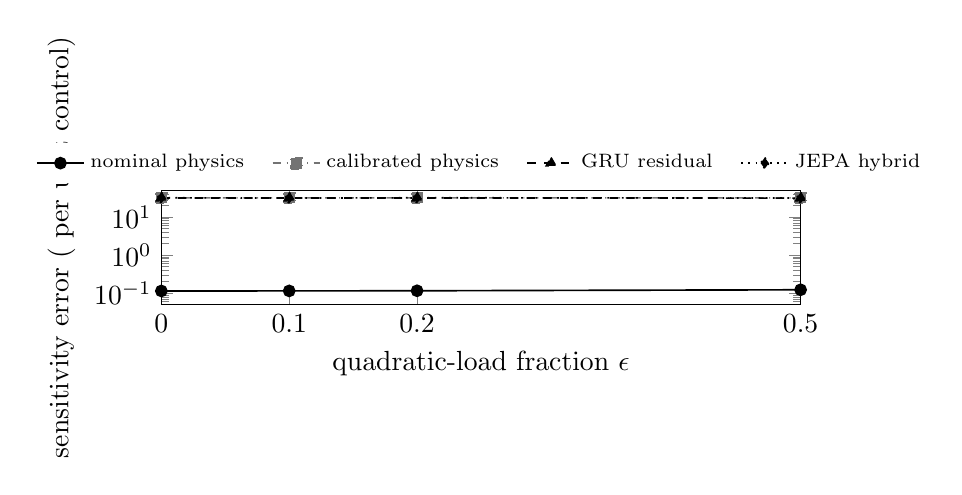
\begin{tikzpicture}
\begin{axis}[width=0.80\textwidth,height=0.25\textwidth, xlabel={quadratic-load fraction $\epsilon$}, ylabel={sensitivity error (\si{\radian\per\second} per unit control)}, xmin=0,xmax=.5,ymin=.05,ymax=50,ymode=log, xtick={0,.1,.2,.5}, grid=none, minor y tick num=1, legend style={font=\scriptsize, draw=none, at={(0.5,1.06)}, anchor=south, legend columns=4,/tikz/every even column/.append style={column sep=0.8em}}]
  \addplot[black, solid, semithick, mark=*] coordinates {(0,.1138) (.1,.1143) (.2,.1152) (.5,.1223)}; \addlegendentry{nominal physics}
  \addplot[black!55, dashdotted, semithick, mark=square*] coordinates {(0,31.7855) (.1,31.7815) (.2,31.7772) (.5,31.7523)}; \addlegendentry{calibrated physics}
  \addplot[black, dashed, semithick, mark=triangle*] coordinates {(0,31.7166) (.1,31.6814) (.2,31.6369) (.5,31.3821)}; \addlegendentry{GRU residual}
  \addplot[black, dotted, semithick, mark=diamond*] coordinates {(0,32.0246) (.1,31.5194) (.2,32.0010) (.5,31.6104)}; \addlegendentry{JEPA hybrid}
\end{axis}
\end{tikzpicture}
